\begin{figure}[!htbp]
    \centering
    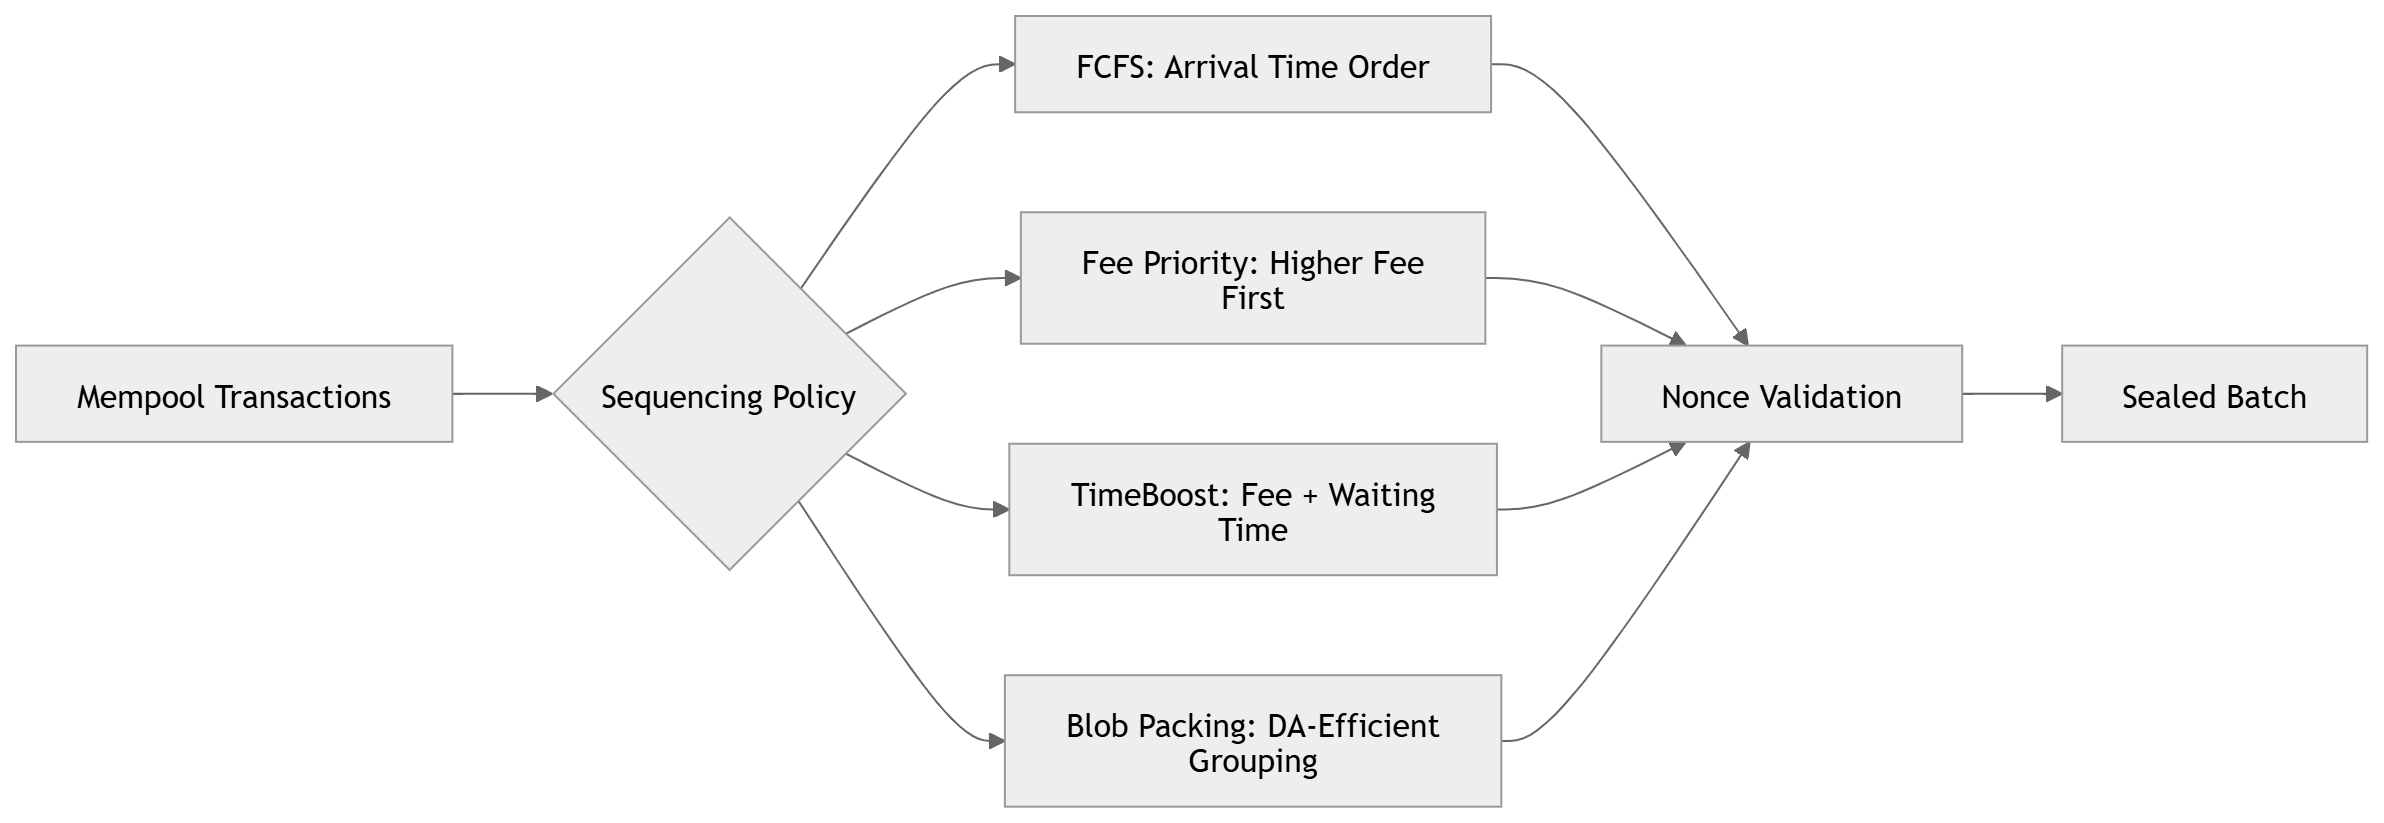
\includegraphics[
        width=0.82\textwidth,
        keepaspectratio
    ]{figures/chapter3/seq_policy.png}
    \caption{Sequencing-policy comparison flow.}
    \label{fig:sequencing_policy_flow}
\end{figure}

\subsection{Sequencing Policy Space} \label{subsec:sequencing_policy_space} Sequencing determines the order in which transactions are selected from the transaction pool and placed into a sealed batch. The implementation uses the Strategy pattern so that different scheduling policies can be selected without changing the core batching logic. This makes the Sequencer suitable for controlled experiments where the same workload can be tested under different transaction ordering rules. A key rule in the implementation is that forced Layer-1 transactions are always placed at the beginning of the batch. This rule is applied regardless of the selected sequencing policy. The sequencing policy only controls the ordering of normal pooled transactions after forced transactions have been handled. This separation preserves forced-inclusion ordering while still allowing the framework to evaluate different scheduling strategies for ordinary Layer-2 traffic. \begin{table}[!htbp] \centering \caption{Sequencing Policy Configuration Space} \label{tab:sequencing_policy_space} \compacttable \begin{tabularx}{\textwidth}{@{}p{0.22\textwidth}Y Y@{}} \toprule \textbf{Policy} & \textbf{Ordering rule} & \textbf{Benchmarking purpose} \\ \midrule FCFS & Preserves the original transaction arrival order without reordering normal transactions. & Provides the baseline policy for measuring throughput, latency, and fairness under simple first-come-first-served behaviour. \\ \addlinespace FeePriority & Sorts transactions by \texttt{gas\_price} in descending order. Transactions offering higher fees are placed earlier in the batch. & Allows evaluation of revenue-oriented ordering and its effect on latency distribution during high-load periods. \\ \addlinespace TimeBoost & Groups transactions into discrete time windows, controlled by \texttt{time\_window\_ms}. Within the same window, transactions are ordered by \texttt{boost\_bid}, then by \texttt{gas\_price}, with FCFS used as a tie-breaker. & Provides a hybrid fairness and priority mechanism, allowing the study to observe how time-windowed priority affects latency and ordering fairness. \\ \addlinespace FairBFT & Sorts transactions by timestamp in ascending order. Older transactions are prioritized before newer transactions. & Models a fairness-oriented ordering policy that reduces opportunities for front-running in a single-node experimental sequencer. \\ \addlinespace BlobPacking & Sorts transactions primarily by encoded payload size in descending order, followed by \texttt{gas\_price} and timestamp as secondary criteria. & Optimizes batch construction for blob utilization and is useful for evaluating EIP-4844-oriented data availability efficiency. \\ \bottomrule \end{tabularx} \end{table} 
ormalsize The FCFS policy is used as the default baseline because it preserves transaction arrival order and introduces minimal scheduling logic. FeePriority allows the benchmark to study how fee-based ordering affects user latency and batch composition. TimeBoost introduces a more nuanced policy by combining time-window fairness with priority bids and gas price. FairBFT provides a simplified fairness-oriented policy by ordering transactions according to timestamp. BlobPacking is designed specifically for data availability experiments, where the objective is to improve blob fill efficiency before timeout-based sealing occurs. These sequencing policies allow the framework to evaluate how transaction ordering influences system behaviour under different workload conditions. Under low load, different policies may produce similar throughput but different fairness properties. Under high load, policies such as FeePriority and BlobPacking may significantly change latency distribution, batch composition, and data availability utilization. Therefore, sequencing policy is treated as a major experimental variable alongside batching policy, prover mode, and data availability mode. Together, the batching and sequencing configuration spaces define how the Sequencer transforms incoming transaction traffic into executable batches. This makes them central to the project’s methodology, because they directly affect queueing delay, batch size distribution, throughput, finalization time, and cost per transaction.